\section{NVIDIA Jetson TK1 development board}
\label{sec:jetson_tk1}

Στο κεφάλαιο αυτό παρουσιάζεται η ενσωματωμένη πλατφόρμα Jetson TK1 της NVIDIA,
η οποία χρησιμοποιήθηκε για εφαρμογή των υλοποιήσεων για
\emph{Αναγνώριση και Εντοπισμό Αντικειμένων} σε συστήματα πραγματικού χρόνου,
με Νευρωνικά Δίκτυα Συνέλιξης.

Ο \emph{Tegra K1} είναι το πρώτο SOC της NVIDIA, για φορητές συσκευές, με προηγμένη αρχιτεκτονική
και χαρακτηριστικά, καθώς και χαμηλή κατανάλωση ισχύως. H μέγιστη κατανάλωση είναι στα \emph{3 Watt},
τιμή που δικαιολογεί την ενσωμάτωση του σε φορητές συσκευές (tablets, smartphones), καθώς και
σε προηγμένα ενσωματωμένα συστήματα (embedded systems) για εφαρμογές πραγματικού χρόνου.
\begin{figure}[H]
  \centering
  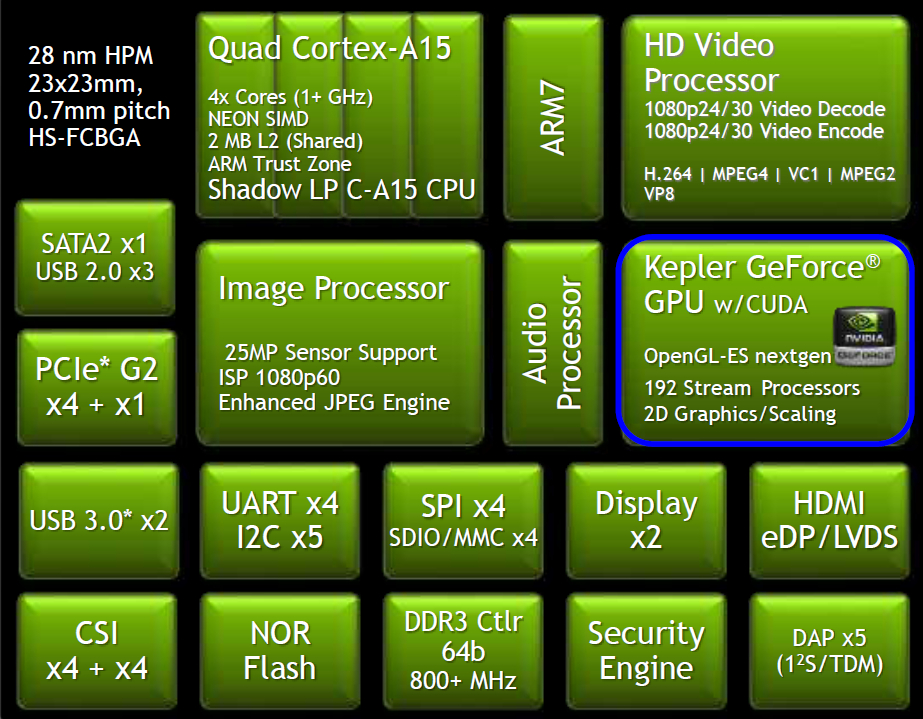
\includegraphics[width=0.7\textwidth]{./images/chapter4/nvidia_tegrak1_block2.jpg}
  \caption{Tegra K1 SOC}
  \label{fig:tegrak1soc}
\end{figure}
\noindent
Όπως φαίνεται στο \autoref{fig:tegrak1soc}, τα βασικά τεχνικά χαρακτηριστικά του Tegra K1 SOC:
\begin{itemize}
  \item{CPU: Quad-core ARM Cortex-A15 CPU, 2.3Ghz}
  \item{GPU: GK20A Kepler-based GPU with 192 CUDA cores}
  \item{RAM: DDR3L/LPDDR3, up to 8GB}
  \item{Peripherals I/O: USB, eMMC/SD-card, LVDS, HDMI, SPI, UART, I2C, SATA, PCIe}
  \item{ISP: Image processor}
\end{itemize}

Στα πλαίσια της παρούσας διπλωματικής εργασίας, επιλέκτηκε να χρησιμοποιή-σουμε το
\emph{Jetson TK1} development board της NVIDIA.
\begin{figure}[!ht]
  \centering
  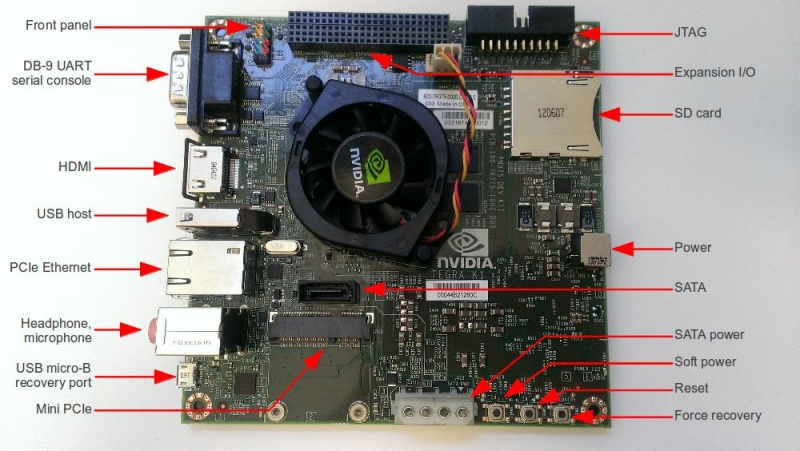
\includegraphics[width=0.9\textwidth]{./images/chapter5/jetson-tk1-labelled.jpg}
  \caption[Jetson TK1 development board]{Jetson TK1 development board}
\end{figure}
Το Jetson TK1 ενσωματώνει το Tegra K1 SOC (CPU+GPU+ISP)
και είναι πλήρες συμβατό με διάφορες διανομές λειτουργικών συστημάτων Linux (Ubuntu, Debian, Arch, Fedora, openSUSE, Gentoo).
Η πλήρες σθμβατότητα και υποστήριξη λειτουργικού συστήματος Linux ήταν βασικό κριτήριο
στην επιλογή του συγκεκριμένου ενσωματωμένου συστήματος αφού επιτρέπει την
εγκατάσταση εργαλείων με τον ίδιο τρόπο όπως σε ένα σταθερό υπολογιστικό σύστημα (Desktop PC)
το οποίο τρέχει Linux OS. Πέρα από την συμβατότητα με κλασσικές διανομές Linux OS,
η NVIDIA έχει αναπτύξει δικό της λειτουργικό σύστημα, \emph{Linux4Tegra}, το οποίο
έχει σαν βάση τα Ubuntu-14.04, με κάποιες επεκτάσεις για πλήρη υποστήριξη του hardware του Jetson TK1.
Επιπλέον παράγοντας στην επιλογή της συγκεκριμένης πλατφόρμας είναι η πληθώρα των περιφερειακων διεπαφών που
διαθέτει, κάνοντας το χρήσιμο για εφαρμογή σε ρομποτικά συστήματα όπου η σύνδεση διαφόρων περιφεριακών συσκευών,
όπως για παράδειγμα αισθητήρες, κάμερες, κινητήρες, σερβο-κινητήρες, είναι απαίτηση.
Πιο κάτω δίνονται οι βασικές διεπαφές που προσφέρει η πλατφόρμα Jetson TK1:
\begin{itemize}
  \item{mini-PCIe: Σύνδεση πρόσθετων συσκευών στον δίαυλο PCI-Express όπως, Wifi cards, SSD δίσκων, κτλ.}
  \item{USB 2.0 port: Για σύνδεση συσκευών ή/και αισθητήρων με διεπαφή eHCI (Extended Host Controller Interface)}
  \item{USB 3.0 port: Για σύνδεση συσκευών ή/και αισθητήρων με διεπαφή xHCI (eXtensible Host Controller Interface)}
  \item{HDMI: Δίνει την δυνατότητα σύνδεσης οθόνης}
  \item{RS232 port: Παρόλο που το RS232 είναι αρκετά παλιό προτόκολο επκοινωνίας, ακόμη ενσωματώνεται σε διάφορες συσκευές που δεν απαιτούν μεγάλο όγκο μεταφοράς δεδομένων, όπως οι οδηγοί κινητήρων}
  \item{Audio IO}
  \item{Gigabit Ethernet LAN: Δικτύωση της πλατφόρμας με τον "έξω" κόσμο}
  \item{SATA: Επιτρέπει την σύνδεση σκληρού δίσκου SATA}
  \item{JTAG port: Το JTAG προσφέρει την δυνατότητα σύνδεσης συσκευής/προγράμματος εντοπισμού σφαλμάτων (debugger), για επαγγελματική αποσφαλμάτωση}
  \item{UART port}
  \item{I2C ports: Διαθέτει τρείς θύρες I2C για σύνδεση αισθητήρων/συσκευών που οδηγούνται με το συγκεκριμένο προτόκολο}
  \item{GPIO: Προσφέρει δύο θυρες επέκτασης (expansion ports), με 50 και 75 ακροδέκτες αντίστοιχα. Χρησιμο κυρίως για, επικοινωνία συσκευών με SPI, οδήγηση σερβο-κινητήρων, διακλάδωση τροφοδοσίας σε τρίτες συσκευές, κτλ.}
\end{itemize}

Όσον αφορά την υλοποίηση και ανάπτυξη Νευρωνικών Δικτύων σε ενσωματωμένα συστήματα, το Jetson TK1 θεωρείτε ιδανικό
αφού υποστηρίζει CUDA και cuDNN. H cuDNN (CUDA Deep Neural Network library) είναι GPU-accelerated βιβλιοθήκη για Νευρωνικά Δίκτυα,
η οποία αναπτύχθηκε από την NVIDIA και προσφέρει υψηλού επιπέδου υλοποιήσεις για ρουτίνες όπως συνέλιξη, κανονικοποίηση δεδομένων, pooling, επίπεδα ενεργοποίησης, κτλ.
Η βιβλιοθήκη cuDNN χρησιμοποιέιτε και ενσωματώνετε σε όλα τα frameworks βαθιας εκμάθησης, όπως Caffe \cite{jia2014caffe}, Tensorflow \cite{DBLP:journals/corr/AbadiBCCDDDGIIK16}, Theano \cite{2016arXiv160502688full}\cite{bergstra+al:2010-scipy}\cite{Bastien-Theano-2012}, Torch \cite{collobert2002torch}\cite{collobert2011torch7}\cite{collobert2012implementing}, CNTΚ και Keras.
